\section{Introducción}

  \DEF{Software} Colección de programas,  procedimientos, y la documentación y   datos asociados que determinan la
  operación de un sistema de computación.

  \PN\DEF{Dominio del problema}

  \begin{center}
    \begin{tabular}{ | l | c | r | }
      \hline
                                & Alumno          & Industria \\ \hline
      Error (bug)               & Tolerable       & No Tolerable \\ \hline
      Interfaz                  & No importante   & Muy importante \\ \hline
      documentación             & No existe       & Existe: Usuario y proyecto \\ \hline
      Confiabilidad y robustez  & No importante   & Fundamental \\ \hline
      Inversión                 & No Existe       & Fuerte \\ \hline
      Portabilidad              & No importante   & Clave \\ \hline
    \end{tabular}
  \end{center}

  \PN En software las \textit{fallas} \textcolor{red}{NO} son consecuencia del uso y el deterioro. Las fallas ocurren
    como consecuencia de errores introducidos durante el desarrollo.

  \PN\DEF{Mantenimiento}
  \begin{itemize}
    \item \textbf{Correctivo} (updates) errores.
    \item \textbf{Adaptativo} (upgrade) funcionalidad.
  \end{itemize}

  \PN\DEF{Ingeniería de Software} Aplicación de un enfoque sistemático,
  disciplinado, y cuantificable al desarrollo, operación, y
  mantenimiento del software.

  \PN\DEF{Enfoque sistemático} Metodología y prácticas existentes para solucionar un problema dentro de un dominio
  determinado. Esto permite repetir el proceso y da la posibilidad de predecirlo (independientemente del grupo de 
  personas que lo lleva a cabo).

  \PN\DEF{Factor principal} Satisfacer necesidades cliente/usuario
  
  \PN\DEF{Factores de impacto}
  \begin{itemize}
    \item \textbf{Escala:} Debe funcionar para entradas pequeñas y grandes.
    \item \textbf{Productividad:} Reducir las \textit{KLOC/PM}.
    \item \textbf{Calidad:} Densidad de defectos (\textit{\#defectos / tamaño}) (+ fallas $\Rightarrow$ - confiable)
          \begin{itemize} 
            \item \textbf{Funcionalidad}  Capacidad de proveer funciones que cumplen las necesidades establecidas o
                                          implicadas.
            \item \textbf{Confiabilidad}  Capacidad de realizar las funciones requeridas bajo las condiciones 
                                          establecidas durante un tiempo específico.
            \item \textbf{Usabilidad}     Capacidad de ser comprendido, aprendido y usado.
            \item \textbf{Eficiencia}     Capacidad de proveer desempeño apropiado relativo a la cantidad de recursos
                                          usados.
            \item \textbf{Mantenibilidad} Capacidad de ser modificado con el propósito de corregir, mejorar, o adaptar.
            \item \textbf{Portabilidad}   Capacidad de ser adaptado a distintos entornos sin aplicar otras acciones que
                                          las provistas a este propósito en el producto.
          \end{itemize}
    \item \textbf{Consistencia y repetitividad:}  Sucesiva producción de sistemas de alta calidad y con alta
                                                  productividad que pueda ser repetido.
    \item \textbf{Cambio:} Adaptarse a las necesidades.
  \end{itemize}

  \PN\textbf{\underline{Triángulo de hierro:}}

  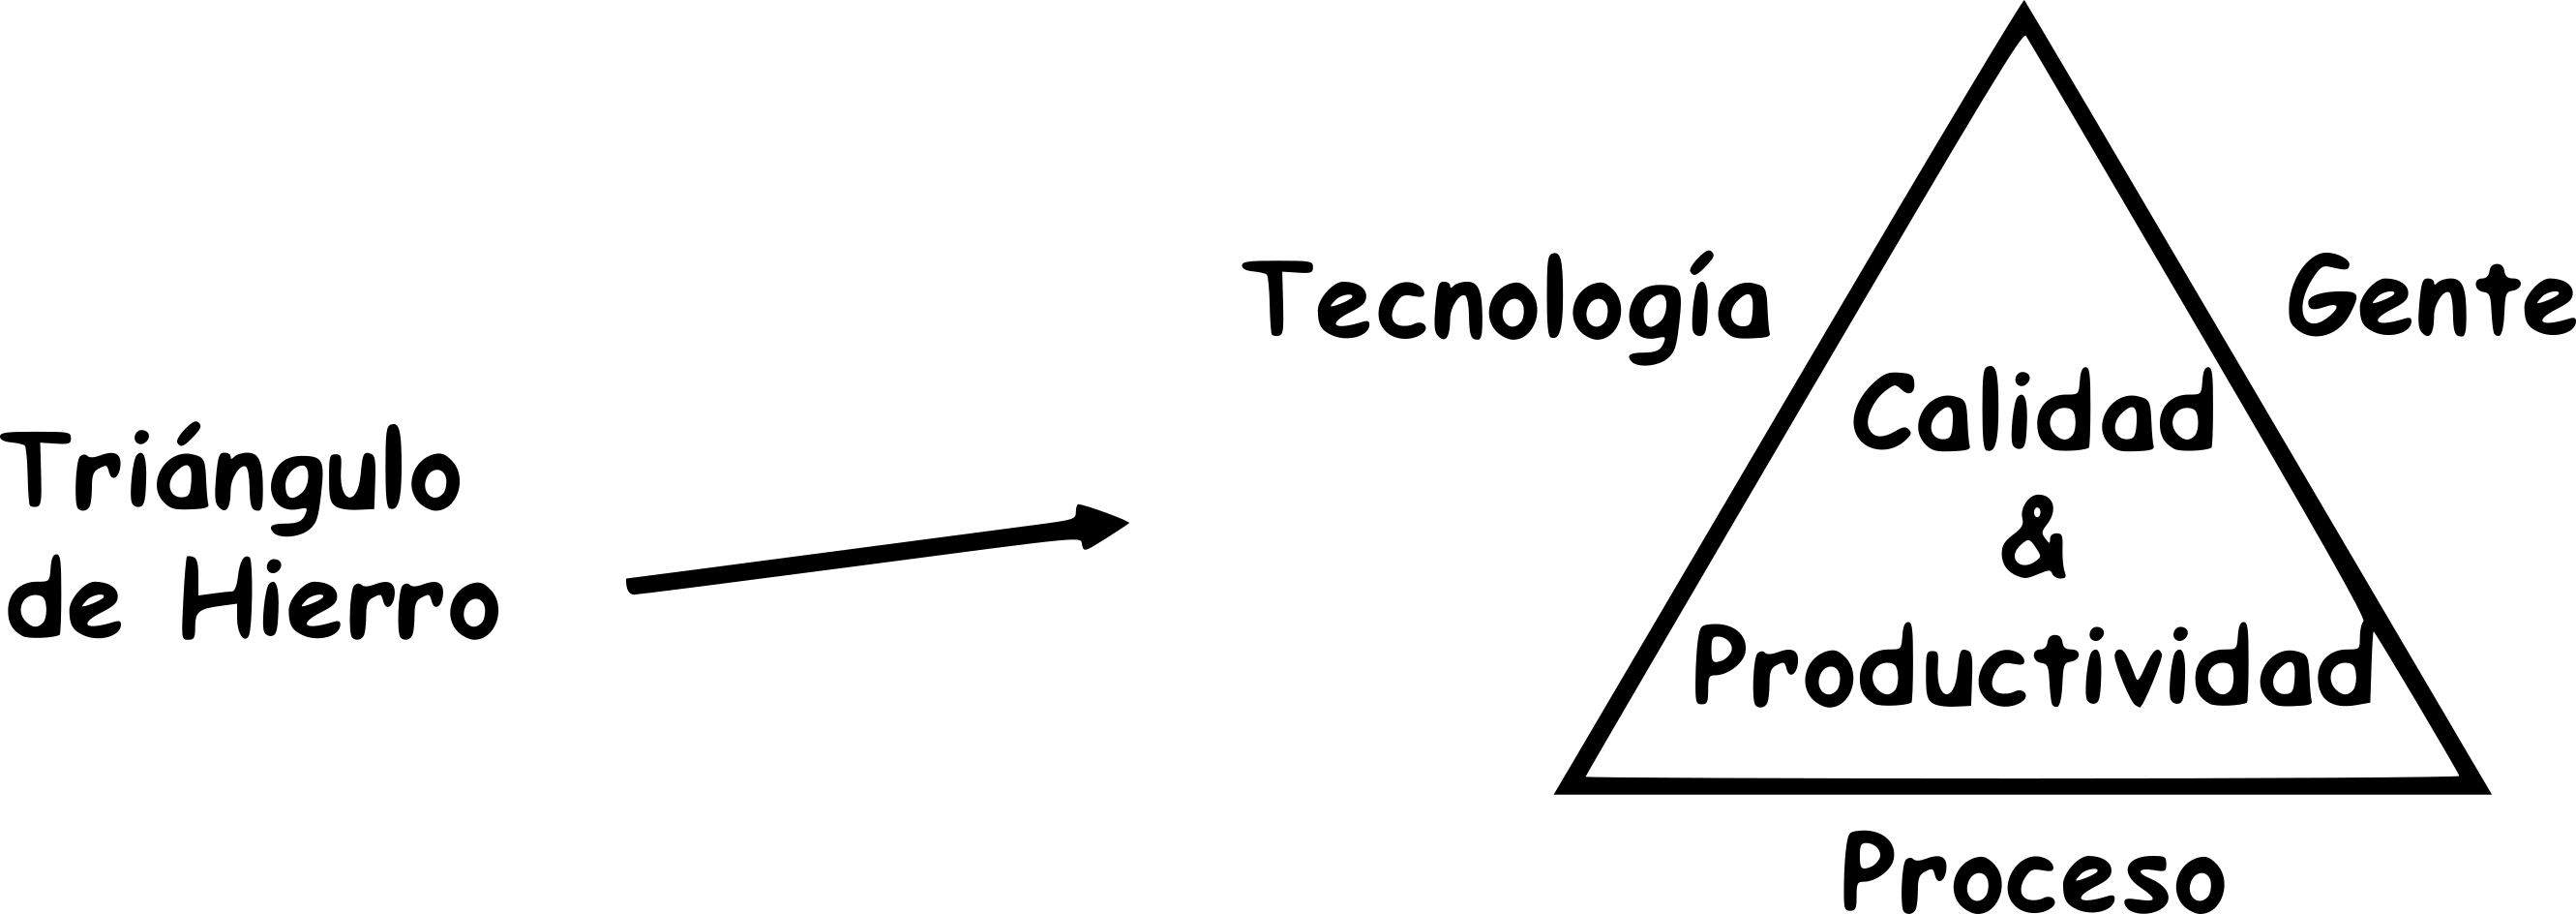
\includegraphics[scale=0.4]{graphics/figure_1.png}

  \PN\DEF{Fases del proceso de desarrollo}
  \begin{itemize}
    \item \textbf{Análisis de requisitos y especificación}
    \item \textbf{Arquitectura y Diseño}
    \item \textbf{Codificación}
    \item \textbf{Testing}
    \item \textbf{Entrega e instalación}
  \end{itemize}

  \pagebreak